\paragraph{QuizziPedia::Front-End::ModelViews::ResultsModelView}
	
	\label{QuizziPedia::Front-End::ModelViews::ResultsModelView}
	
	\begin{figure}[ht]
		\centering
		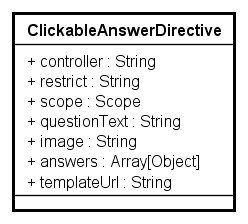
\includegraphics[scale=0.5,keepaspectratio]{UML/Classi/Front-End/QuizziPedia_Front-end_Templates_ClickableAnswerTemplate.png}
		\caption{QuizziPedia::Front-End::ModelViews::ResultsModelView}
	\end{figure} \FloatBarrier
	
	\begin{itemize}
		\item \textbf{Descrizione}: classe di tipo modelview la cui istanziazione è contenuta all'interno della variabile di ambiente \$scope di \textit{Angular.js\ped{G}}. All'interno di essa sono presenti le variabili e i metodi necessari per il \textit{Two-Way Data-Binding\ped{G}} tra la view \texttt{ResultsView} e il controller \texttt{ResultsController};
		\item \textbf{Utilizzo}: viene utilizzata per effettuare il \textit{Two-Way Data-Binding\ped{G}} tra la view \texttt{ResultsView} e il controller \texttt{ResultsController} rendendo disponibili variabili e metodi;
		\item \textbf{Relazioni con altre classi}: 
		\begin{itemize}
			\item \textit{IN} \texttt{ResultsView}: view contenente i risultati della ricerca effettuata, sia gli utenti che i questionari trovati; 
			\item \textit{IN} \texttt{SearchController}: questa classe permette di gestire la ricerca di questionari e utenti all’interno dell’applicazione;
		\end{itemize}
		\item \textbf{Attributi}: 
		\begin{itemize}
			\item \texttt{+ username: String} \\ Attributo che conterrà l'username dell'utente ricercato;
			\item \texttt{+ name: String} \\ Attributo che conterrà il nome del questionario ricercato;
			\item \texttt{+ author: String} \\ Attributo che conterrà l'autore del questionario ricercato;
			\item \texttt{+ topic: String} \\ Attributo che conterrà l'argomento del questionario ricercato;
			\item \texttt{+ keywords: String} \\ Attributo che conterrà le keywords del questionario ricercato.
		\end{itemize}
		\item \textbf{Metodi}: 
		\begin{itemize}
				\item \texttt{+} \texttt{goToUser(idUser: String): void} \\
				Metodo che gestisce l’evento click sul bottone per visualizzare il profilo dell'utente selezionato. Effettua il redirect alla pagina dell'utente.\\
				\textbf{Parametri}:
				\begin{itemize}
					\item \texttt{idUser: String} \\
					Parametro contenente l'id dell'utente di cui si vuole visualizzare il profilo;
				\end{itemize} 
				\item \texttt{+} \texttt{registrationToQuiz(idQuiz: String): void} \\
				Metodo che gestisce l’evento click sul pulsante di registrazione al questionario.\\
				\textbf{Parametri}:
				\begin{itemize}
					\item \texttt{idQuiz: String} \\
					Parametro contenente l'id del questionario di cui si vuole effettuare l'iscrizione;
				\end{itemize} 
				\item \texttt{+} \texttt{goToResultsPage(stringSearch: String): void} \\
				Metodo che gestisce l’evento click sul pulsante per effettuare una ricerca.\\
				\textbf{Parametri}:
				\begin{itemize}
					\item \texttt{stringSearch: String} \\
					Parametro contenente la stringa della quale effettuare la ricerca;
				\end{itemize} 
		\end{itemize}
	\end{itemize}

	